\documentclass[12pt]{article}

\usepackage{amsmath, mathtools}
\usepackage{amsfonts}
\usepackage{amssymb}
\usepackage{graphicx}
\usepackage{colortbl}
\usepackage{xr}
\usepackage{hyperref}
\usepackage{longtable}
\usepackage{xfrac}
\usepackage{tabularx}
\usepackage{float}
\usepackage{siunitx}
\usepackage{booktabs}
\usepackage{caption}
\usepackage{pdflscape}
\usepackage{afterpage}
\usepackage{enumerate}
\usepackage[shortlabels]{enumitem}

\usepackage[round]{natbib}

%\usepackage{refcheck}

\hypersetup{
    bookmarks=true,         % show bookmarks bar?
      colorlinks=true,       % false: boxed links; true: colored links
    linkcolor=red,          % color of internal links (change box color with linkbordercolor)
    citecolor=green,        % color of links to bibliography
    filecolor=magenta,      % color of file links
    urlcolor=cyan           % color of external links
}

%% Comments

\usepackage{color}

\newif\ifcomments\commentstrue %displays comments
%\newif\ifcomments\commentsfalse %so that comments do not display

\ifcomments
\newcommand{\authornote}[3]{\textcolor{#1}{[#3 ---#2]}}
\newcommand{\todo}[1]{\textcolor{red}{[TODO: #1]}}
\else
\newcommand{\authornote}[3]{}
\newcommand{\todo}[1]{}
\fi

\newcommand{\wss}[1]{\authornote{blue}{SS}{#1}} 
\newcommand{\plt}[1]{\authornote{magenta}{TPLT}{#1}} %For explanation of the template
\newcommand{\an}[1]{\authornote{cyan}{Author}{#1}}

%% Common Parts

\newcommand{\progname}{Software Engineering} % PUT YOUR PROGRAM NAME HERE
\newcommand{\authname}{Team 16, Durum Wheat Semolina
	\\ Alexander Moica
	\\ Yasmine Jolly
	\\ Jeffrey Wang
	\\ Jack Theriault
	\\ Catherine Chen
	\\ Justina Srebrnjak } % AUTHOR NAMES                 

\usepackage{hyperref}
    \hypersetup{colorlinks=true, linkcolor=blue, citecolor=blue, filecolor=blue,
                urlcolor=blue, unicode=false}
    \urlstyle{same}
                                


% For easy change of table widths
\newcommand{\colZwidth}{1.0\textwidth}
\newcommand{\colAwidth}{0.13\textwidth}
\newcommand{\colBwidth}{0.82\textwidth}
\newcommand{\colCwidth}{0.1\textwidth}
\newcommand{\colDwidth}{0.05\textwidth}
\newcommand{\colEwidth}{0.8\textwidth}
\newcommand{\colFwidth}{0.17\textwidth}
\newcommand{\colGwidth}{0.5\textwidth}
\newcommand{\colHwidth}{0.28\textwidth}

% Used so that cross-references have a meaningful prefix
\newcounter{defnum} %Definition Number
\newcommand{\dthedefnum}{GD\thedefnum}
\newcommand{\dref}[1]{GD\ref{#1}}
\newcounter{datadefnum} %Datadefinition Number
\newcommand{\ddthedatadefnum}{DD\thedatadefnum}
\newcommand{\ddref}[1]{DD\ref{#1}}
\newcounter{theorynum} %Theory Number
\newcommand{\tthetheorynum}{T\thetheorynum}
\newcommand{\tref}[1]{T\ref{#1}}
\newcounter{tablenum} %Table Number
\newcommand{\tbthetablenum}{T\thetablenum}
\newcommand{\tbref}[1]{TB\ref{#1}}
\newcounter{assumpnum} %Assumption Number
\newcommand{\atheassumpnum}{P\theassumpnum}
\newcommand{\aref}[1]{A\ref{#1}}
\newcounter{goalnum} %Goal Number
\newcommand{\gthegoalnum}{P\thegoalnum}
\newcommand{\gsref}[1]{GS\ref{#1}}
\newcounter{instnum} %Instance Number
\newcommand{\itheinstnum}{IM\theinstnum}
\newcommand{\iref}[1]{IM\ref{#1}}
\newcounter{reqnum} %Requirement Number
\newcommand{\rthereqnum}{P\thereqnum}
\newcommand{\rref}[1]{R\ref{#1}}
\newcounter{nfrnum} %NFR Number
\newcommand{\rthenfrnum}{NFR\thenfrnum}
\newcommand{\nfrref}[1]{NFR\ref{#1}}
\newcounter{lcnum} %Likely change number
\newcommand{\lthelcnum}{LC\thelcnum}
\newcommand{\lcref}[1]{LC\ref{#1}}
\newcounter{ulcnum} %Unlikely change number
\newcommand{\ltheulcnum}{ULC\theulcnum}
\newcommand{\ulcref}[1]{ULC\ref{#1}}
\newcounter{FRCounter}
\setcounter{FRCounter}{1}
\newcommand{\FillFRNumber}{\textbf{FR\arabic{FRCounter}.} \stepcounter{FRCounter}}

\usepackage{fullpage}

\newcommand{\deftheory}[9][Not Applicable]
{
\newpage
\noindent \rule{\textwidth}{0.5mm}

\paragraph{RefName: } \textbf{#2} \phantomsection 
\label{#2}

\paragraph{Label:} #3

\noindent \rule{\textwidth}{0.5mm}

\paragraph{Equation:}

#4

\paragraph{Description:}

#5

\paragraph{Notes:}

#6

\paragraph{Source:}

#7

\paragraph{Ref.\ By:}

#8

\paragraph{Preconditions for \hyperref[#2]{#2}:}
\label{#2_precond}

#9

\paragraph{Derivation for \hyperref[#2]{#2}:}
\label{#2_deriv}

#1

\noindent \rule{\textwidth}{0.5mm}

}

\begin{document}

\title{Software Requirements Specification for \progname} 
\author{Catherine Chen, Yasmine Jolly,\\ Jeffrey Wang, Jack Theriault,\\ Alex 
Moica, Justina Srebrnjak}
\date{\today}
	
\maketitle

~\newpage

\pagenumbering{roman}

\tableofcontents

~\newpage

\section*{Revision History}

\begin{tabularx}{\textwidth}{p{3cm}p{2cm}X}
\toprule {\bf Date} & {\bf Version} & {\bf Notes}\\
\midrule
\today & 1.0 & Initial Version\\
%Date 2 & 1.1 & Notes\\
\bottomrule
\end{tabularx}

~\newpage

\section{Reference Material}

This section records information for easy reference.

\subsection{Table of Units}

Throughout this document SI (Syst\`{e}me International d'Unit\'{e}s) is employed
as the unit system.  In addition to the basic units, several derived units are
used as described below.  For each unit, the symbol is given followed by a
description of the unit and the SI name.
~\newline

\renewcommand{\arraystretch}{1.2}
%\begin{table}[ht]
  \noindent \begin{tabular}{l l l} 
    \toprule		
    \textbf{symbol} & \textbf{unit} & \textbf{SI}\\
    \midrule 
    \si{\metre} & length & metre\\
    \si{\kilogram} & mass	& kilogram\\
    \si{\second} & time & second\\
    \si{\celsius} & temperature & centigrade\\
    \si{\joule} & energy & joule\\
    \si{\watt} & power & watt (W = \si{\joule\per\second})\\
    \bottomrule
  \end{tabular}
  %	\caption{Provide a caption}
%\end{table}

\plt{Only include the units that your SRS actually uses.}

\plt{Derived units, like newtons, pascal, etc, should show their derivation
    (the units they are derived from) if their constituent units are in the
    table of units (that is, if the units they are derived from are used in the
    document).  For instance, the derivation of pascals as
    $\si{\pascal}=\si{\newton\per\square\meter}$ is shown if newtons and m are
    both in the table.  The derivations of newtons would not be shown if kg and
    s are not both in the table.}

\plt{The symbol for units named after people use capital letters, but the name 
  of the unit itself uses lower case.  For instance, pascals use the symbol Pa,
  watts use the symbol W, teslas use the symbol T, newtons use the symbol N,
  etc.  The one exception to this is degree Celsius.  Details on writing metric
  units can be found on the 
  \href{https://www.nist.gov/pml/weights-and-measures/writing-metric-units}
  {NIST} web-page.}

\subsection{Table of Symbols}

The table that follows summarizes the symbols used in this document along with
their units.  The choice of symbols was made to be consistent with the heat
transfer literature and with existing documentation for solar water heating
systems.  The symbols are listed in alphabetical order.

\renewcommand{\arraystretch}{1.2}
%\noindent \begin{tabularx}{1.0\textwidth}{l l X}
\noindent \begin{longtable*}{l l p{12cm}} \toprule
\textbf{symbol} & \textbf{unit} & \textbf{description}\\
\midrule 
$A_C$ & \si[per-mode=symbol] {\square\metre} & coil surface area
\\
$A_\text{in}$ & \si[per-mode=symbol] {\square\metre} & surface area over 
which heat is transferred in
\\ 
\bottomrule
\end{longtable*}
\plt{Use your problems actual symbols.  The si package is a good idea to use for
  units.}

\subsection{Abbreviations and Acronyms}

\renewcommand{\arraystretch}{1.2}
\begin{tabular}{l l} 
  \toprule		
  \textbf{symbol} & \textbf{description}\\
  \midrule 
  A & Assumption\\
  DD & Data Definition\\
  GD & General Definition\\
  GS & Goal Statement\\
  IM & Instance Model\\
  LC & Likely Change\\
  PS & Physical System Description\\
  R & Requirement\\
  SRS & Software Requirements Specification\\
  T & Theoretical Model\\
  \bottomrule
\end{tabular}\\

\plt{Add any other abbreviations or acronyms that you add}

\subsection{Mathematical Notation}

\plt{This section is optional, but should be included for projects that make use
  of notation to convey mathematical information.  For instance, if typographic
  conventions (like bold face font) are used to distinguish matrices, this
  should be stated here.  If symbols are used to show mathematical operations,
  these should be summarized here.  In some cases the easiest way to summarize
  the notation is to point to a text or other source that explains the
  notation.}

\plt{This section was added to the template because some students use very
  domain specific notation.  This notation will not be readily understandable to
  people outside of your domain.  It should be explained.}

\newpage

\pagenumbering{arabic}

\plt{This SRS template is based on \citet{SmithAndLai2005, SmithEtAl2007}.  It
  will get you started.  You should not modify the section headings, without
  first discussing the change with the course instructor.  Modification means
  you are not following the template, which loses some of the advantage of a
  template, especially standardization.  Although the bits shown below do not
  include type information, you may need to add this information for your
  problem.  If you are unsure, please can ask the instructor.}

\plt{Feel free to change the appearance of the report by modifying the LaTeX
  commands.}

\plt{This template document assumes that a single program is being documented.
  If you are documenting a family of models, you should start with a commonality
  analysis.  A separate template is provided for this.  For program
  families you should look at \cite{Smith2006, SmithMcCutchanAndCarette2017}.
  Single family member programs are often programs based on a single physical
  model.  General purpose tools are usually documented as a family.  Families of
  physical models also come up.}

\plt{The SRS is not generally written, or read, sequentially.  The SRS is a
  reference document.  It is generally read in an ad hoc order, as the need
  arises.  For writing an SRS, and for reading one for the first time, the
  suggested order of sections is:
\begin{itemize}
\item Goal Statement
\item Instance Models
\item Requirements
\item Introduction
\item Specific System Description
\end{itemize}
}

\plt{Guiding principles for the SRS document:
\begin{itemize}
\item Do not repeat the same information at the same abstraction level.  If
  information is repeated, the repetition should be at a different abstraction
  level.  For instance, there will be overlap between the scope section and the
  assumptions, but the scope section will not go into as much detail as the
  assumptions section.
\end{itemize}
}

\plt{The template description comments should be disabled before submitting this
  document for grading.}

\plt{You can borrow any wording from the text given in the template.  It is part
  of the template, and not considered an instance of academic integrity.  Of
  course, you need to cite the source of the template.}

\plt{When the documentation is done, it should be possible to trace back to the
  source of every piece of information.  Some information will come from
  external sources, like terminology.  Other information will be derived, like
  General Definitions.}

\plt{An SRS document should have the following qualities: unambiguous,
  consistent, complete, validatable, abstract and traceable.}

\plt{The overall goal of the SRS is that someone that meets the Characteristics
  of the Intended Reader (Section~\ref{sec_IntendedReader}) can learn,
  understand and verify the captured domain knowledge.  They should not have to
  trust the authors of the SRS on any statements.  They should be able to
  independently verify/derive every statement made.}

\section{Introduction}

\plt{The introduction section is written to introduce the problem.  It starts
  general and focuses on the problem domain. The general advice is to start with
a paragraph or two that describes the problem, followed by a ``roadmap''
paragraph.  A roadmap orients the reader by telling them what sub-sections to
expect in the Introduction section.}

\subsection{Purpose of Document}

This document describes the requirements for 'Utrition'. It will provide a 
detailed overview of the application, and a comprehensive description of the 
software's functional, non-functional requirements, as well as other details 
relevant to the product. The template for this document is a modified version 
of the Volere template \citep{RobertsonAndRobertson2012}.


\plt{This section summarizes the purpose of the SRS document.  It does not focus
  on the problem itself.  The problem is described in the ``Problem
  Description'' section (Section~\ref{Sec_pd}).  The purpose is for the document
  in the context of the project itself, not in the context of this course.
  Although the ``purpose'' of the document is to get a grade, you should not
  mention this.  Instead, ``fake it'' as if this is a real project.  The purpose
  section will be similar between projects.  The purpose of the document is the
  purpose of the SRS, including communication, planning for the design stage,
  etc.}

\subsection{Scope of Requirements} 
When considering the files the user uploads to the system, the requirements of 
this document are constrained to consider only a subset of all possible file 
types. Furthermore, requirements are created under the impression that files 
are of a manageable size. Lastly, we assume the user accesses the system 
through a computer capable of running most modern applications. That is to say, 
the user possesses sufficient hardware capabilities to run the system.

\plt{Modelling the real world requires simplification.  The full complexity of
  the actual physics, chemistry, biology is too much for existing models, and
  for existing computational solution techniques.  Rather than say what is in
  the scope, it is usually easier to say what is not.  You can think of it as
  the scope is initially everything, and then it is constrained to create the
  actual scope.  For instance, the problem can be restricted to 2 dimensions, or
  it can ignore the effect of temperature (or pressure) on the material
  properties, etc.}  

\plt{The scope section is related to the assumptions section
  (Section~\ref{sec_assumpt}).  However, the scope and the assumptions are not
  at the same level of abstraction.  The scope is at a high level.  The focus is
  on the ``big picture'' assumptions.  The assumptions section lists, and
  describes, all of the assumptions.}

\subsection{Characteristics of Intended Reader} \label{sec_IntendedReader}
This document is intended for the developers and testers working on this 
system, so that the requirements of the system can be communicated throughout 
the development process. Readers should have an understanding of the software 
design life cycle as well as the ability to read discrete math at a 
university-level or better in order to fully understand the contents and 
equations used in this document.

\plt{This section summarizes the skills and knowledge of the readers of the
  SRS.  It does NOT have the same purpose as the ``User Characteristics''
  section (Section~\ref{SecUserCharacteristics}).  The intended readers are the
  people that will read, review and maintain the SRS.  They are the people that
  will conceivably design the software that is intended to meet the
  requirements.  The user, on the other hand, is the person that uses the
  software that is built.  They may never read this SRS document.  Of course,
  the same person could be a ``user'' and an ``intended reader.''}

\plt{The intended reader characteristics should be written as unambiguously and
  as specifically as possible.  Rather than say, the user should have an
  understanding of physics, say what kind of physics and at what level.  For
  instance, is high school physics adequate, or should the reader have had a
  graduate course on advanced quantum mechanics?}

\subsection{Organization of Document}

The rest of the SRS will discuss the purpose and context of the system, 
followed by the functional requirements it must satisfy. Then the document will 
mention its non-functional requirements, providing justifications for each. 
This is followed by a discussion of potential issues that may arise during the 
project's development. Lastly, the document lists likely and unlikely 
changes, and includes a traceability matrix for the system.

\plt{This section provides a roadmap of the SRS document.  It will help the
  reader orient themselves.  It will provide direction that will help them
  select which sections they want to read, and in what order.  This section will
  be similar between project.}

\section{General System Description}

This section provides general information about the system.  It identifies the
interfaces between the system and its environment, describes the user
characteristics and lists the system constraints.  \plt{This text can likely be
  borrowed verbatim.}

\plt{The purpose of this section is to provide general information about the
  system so the specific requirements in the next section will be easier to
  understand. The general system description section is designed to be
  changeable independent of changes to the functional requirements documented in
  the specific system description. The general system description provides a
  context for a family of related models.  The general description can stay the
  same, while specific details are changed between family members.}

\subsection{System Context}

\plt{Your system context will include a figure that shows the abstract view of
  the software.  Often in a scientific context, the program can be viewed
  abstractly following the design pattern of Inputs $\rightarrow$ Calculations
  $\rightarrow$ Outputs.  The system context will therefore often follow this
  pattern.  The user provides inputs, the system does the calculations, and then
  provides the outputs to the user.  The figure should not show all of the
  inputs, just an abstract view of the main categories of inputs (like material
  properties, geometry, etc.).  Likewise, the outputs should be presented from
  an abstract point of view.  In some cases the diagram will show other external
  entities, besides the user.  For instance, when the software product is a
  library, the user will be another software program, not an actual end user.
  If there are system constraints that the software must work with external
  libraries, these libraries can also be shown on the System Context diagram.
  They should only be named with a specific library name if this is required by
  the system constraint.}

\begin{figure}[h!]
\begin{center}
 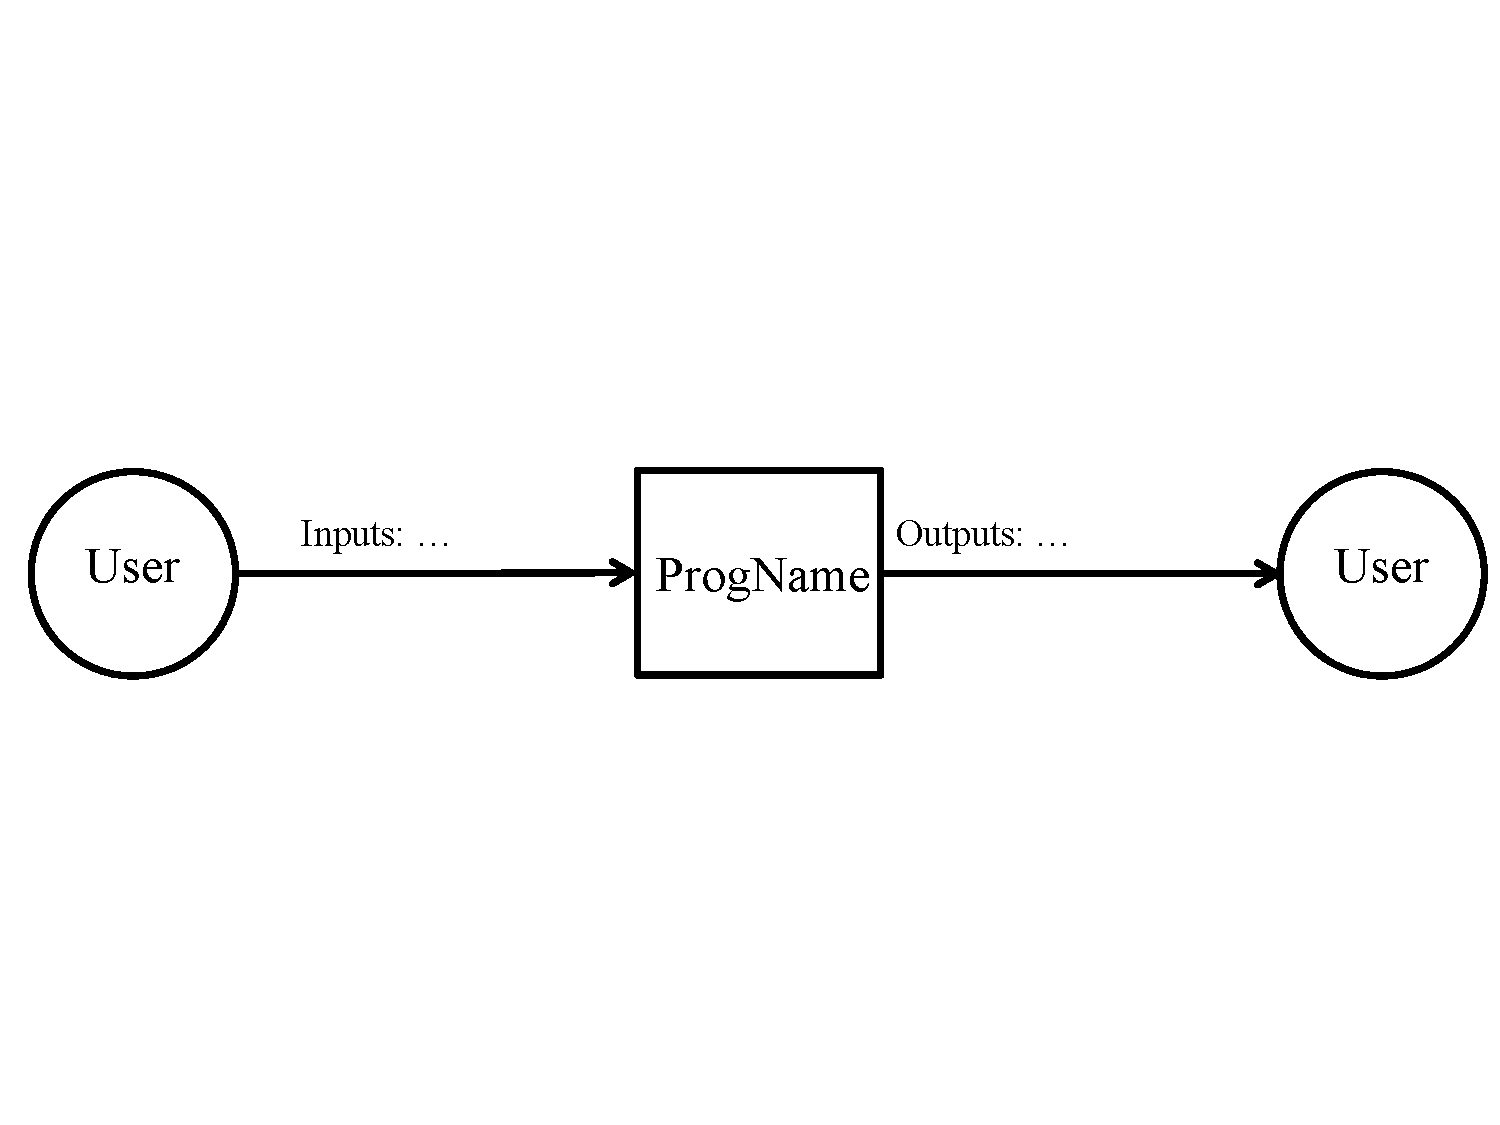
\includegraphics[width=0.6\textwidth]{SystemContextFigure}
\caption{System Context}
\label{Fig_SystemContext} 
\end{center}
\end{figure}

\plt{For each of the entities in the system context diagram its responsibilities
  should be listed.  Whenever possible the system should check for data quality,
  but for some cases the user will need to assume that responsibility.  The list
  of responsibilites should be about the inputs and outputs only, and they
  should be abstract.  Details should not be presented here.  However, the
  information should not be so abstract as to just say ``inputs'' and
  ``outputs''.  A summarizing phrase can be used to characterize the inputs.
  For instance, saying ``material properties'' provides some information, but it
  stays away from the detail of listing every required properties.}

\begin{itemize}
\item User Responsibilities:
\begin{itemize}
\item 
\end{itemize}
\item \progname{} Responsibilities:
\begin{itemize}
\item Detect data type mismatch, such as a string of characters instead of a
  floating point number
\item 
\end{itemize}
\end{itemize}

\subsection{User Characteristics} \label{SecUserCharacteristics}

\plt{This section summarizes the knowledge/skills expected of the user.
  Measuring usability, which is often a required non-function requirement,
  requires knowledge of a typical user.  As mentioned above, the user is a
  different role from the ``intended reader,'' as given in
  Section~\ref{sec_IntendedReader}.  As in Section~\ref{sec_IntendedReader}, the
  user characteristics should be specific an unambiguous.  For instance, ``The
  end user of \progname{} should have an understanding of undergraduate Level 1
  Calculus and Physics.''}

\subsection{System Constraints}

\plt{System constraints differ from other type of requirements because they
  limit the developers' options in the system design and they identify how the
  eventual system must fit into the world. This is the only place in the SRS
  where design decisions can be specified.  That is, the quality requirement for
  abstraction is relaxed here.  However, system constraints should only be
  included if they are truly required.}

\section{Specific System Description}

This section first presents the problem description, which gives a high-level
view of the problem to be solved.  This is followed by the solution characteristics
specification, which presents the assumptions, theories, definitions and finally
the instance models.  \plt{Add any project specific details that are relevant
  for the section overview.}

\subsection{Problem Description} \label{Sec_pd}

\progname{} is intended to solve ... \plt{What problem does your program solve?
The description here should be in the problem space, not the solution space.}

\subsubsection{Terminology and  Definitions}

\plt{This section is expressed in words, not with equations.  It provide the
  meaning of the different words and phrases used in the domain of the problem.
The terminology is used to introduce concepts from the world outside of the
mathematical model  The terminology provides a real world connection to give the
mathematical model meaning.}

This subsection provides a list of terms that are used in the subsequent
sections and their meaning, with the purpose of reducing ambiguity and making it
easier to correctly understand the requirements:

\begin{itemize}

\item 

\end{itemize}

\subsubsection{Physical System Description} \label{sec_phySystDescrip}

\plt{The purpose of this section is to clearly and unambiguously state the
  physical system that is to be modelled. Effective problem solving requires a
  logical and organized approach. The statements on the physical system to be
  studied should cover enough information to solve the problem. The physical
  description involves element identification, where elements are defined as
  independent and separable items of the physical system. Some example elements
  include acceleration due to gravity, the mass of an object, and the size and
  shape of an object. Each element should be identified and labelled, with their
  interesting properties specified clearly. The physical description can also
  include interactions of the elements, such as the following: i) the
  interactions between the elements and their physical environment; ii) the
  interactions between elements; and, iii) the initial or boundary conditions.}

The physical system of \progname{}, as shown in Figure~?,
includes the following elements:

\begin{itemize}

\item[PS1:] 

\item[PS2:] ...

\end{itemize}

\plt{A figure here makes sense for most SRS documents}

% \begin{figure}[h!]
% \begin{center}
% %\rotatebox{-90}
% {
%  \includegraphics[width=0.5\textwidth]{<FigureName>}
% }
% \caption{\label{<Label>} <Caption>}
% \end{center}
% \end{figure}

\subsubsection{Goal Statements}

\plt{The goal statements refine the ``Problem Description''
  (Section~\ref{Sec_pd}).  A goal is a functional objective the system under
  consideration should achieve. Goals provide criteria for sufficient
  completeness of a requirements specification and for requirements
  pertinence. Goals will be refined in Section “Instanced Models”
  (Section~\ref{sec_instance}). Large and complex goals should be decomposed
  into smaller sub-goals.  The goals are written abstractly, with a minimal
  amount of technical language.  They should be understandable by non-domain
  experts.}

\noindent Given the \plt{inputs}, the goal statements are:

\begin{itemize}

\item[GS\refstepcounter{goalnum}\thegoalnum \label{G_meaningfulLabel}:] \plt{One
    sentence description of the goal.  There may be more than one.  Each Goal
    should have a meaningful label.}

\end{itemize}

\subsection{Solution Characteristics Specification}

\plt{This section specifies the information in the solution domain of the system
  to be developed. This section is intended to express what is required in
  such a way that analysts and stakeholders get a clear picture, and the
  latter will accept it. The purpose of this section is to reduce the problem
  into one expressed in mathematical terms. Mathematical expertise is used to
  extract the essentials from the underlying physical description of the
  problem, and to collect and substantiate all physical data pertinent to the
  problem.}

\plt{This section presents the solution characteristics by successively refining
  models.  It starts with the abstract/general Theoretical Models (TMs) and
  refines them to the concrete/specific Instance Models (IMs).  If necessary
  there are intermediate refinements to General Definitions (GDs).  All of these
  refinements can potentially use Assumptions (A) and Data Definitions (DD).
  TMs are refined to create new models, that are called GMs or IMs. DDs are not
  refined; they are just used. GDs and IMs are derived, or refined, from other
  models. DDs are not derived; they are just given. TMs are also just given, but
  they are refined, not used.  If a potential DD includes a derivation, then
  that means it is refining other models, which would make it a GD or an IM.}

\plt{The above makes a distinction between ``refined'' and ``used.'' A model is
  refined to another model if it is changed by the refinement. When we change a
  general 3D equation to a 2D equation, we are making a refinement, by applying
  the assumption that the third dimension does not matter. If we use a
  definition, like the definition of density, we aren't refining, or changing
  that definition, we are just using it.}

\plt{The same information can be a TM in one problem and a DD in another.  It is
  about how the information is used.  In one problem the definition of
  acceleration can be a TM, in another it would be a DD.}

\plt{There is repetition between the information given in the different chunks
  (TM, GDs etc) with other information in the document.  For instance, the
  meaning of the symbols, the units etc are repeated.  This is so that the
  chunks can stand on their own when being read by a reviewer/user.  It also
  facilitates reuse of the models in a different context.}

\noindent \plt{The relationships between the parts of the document are show in
  the following figure.  In this diagram ``may ref'' has the same role as
  ``uses'' above.  The figure adds ``Likely Changes,'' which are able to
  reference (use) Assumptions.}

\begin{figure}[H]
  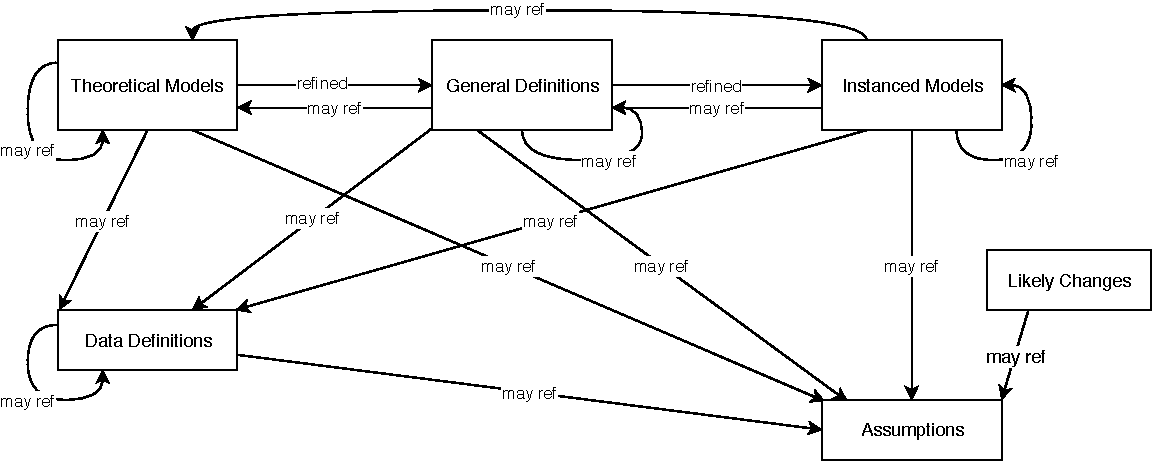
\includegraphics[scale=0.9]{RelationsBetweenTM_GD_IM_DD_A.pdf}
\end{figure}

The instance models that govern \progname{} are presented in
Subsection~\ref{sec_instance}.  The information to understand the meaning of the
instance models and their derivation is also presented, so that the instance
models can be verified.

\subsubsection{Assumptions} \label{sec_assumpt}

\plt{The assumptions are a refinement of the scope.  The scope is general, where
  the assumptions are specific.  All assumptions should be listed, even those
  that domain experts know so well that they are rarely (if ever) written down.}
\plt{The document should not take for granted that the reader knows which
  assumptions have been made. In the case of unusual assumptions, it is
  recommended that the documentation either include, or point to, an explanation
  and justification for the assumption.}

This section simplifies the original problem and helps in developing the
theoretical model by filling in the missing information for the physical
system. The numbers given in the square brackets refer to the theoretical model
[T], general definition [GD], data definition [DD], instance model [IM], or
likely change [LC], in which the respective assumption is used.

\begin{itemize}

\item[A\refstepcounter{assumpnum}\theassumpnum \label{A_meaningfulLabel}:]
  \plt{Short description of each assumption.  Each assumption
    should have a meaningful label.  Use cross-references to identify the
    appropriate traceability to T, GD, DD etc., using commands like dref, ddref
    etc.  Each assumption should be atomic - that is, there should not be an
    explicit (or implicit) ``and'' in the text of an assumption.}

\end{itemize}

\subsubsection{Theoretical Models}\label{sec_theoretical}

\plt{Theoretical models are sets of abstract mathematical equations or axioms
  for solving the problem described in Section ``Physical System Description''
  (Section~\ref{sec_phySystDescrip}). Examples of theoretical models are
  physical laws, constitutive equations, relevant conversion factors, etc.}

This section focuses on the general equations and laws that \progname{} is based
on.  \plt{Modify the examples below for your problem, and add additional models
  as appropriate.}

~\newline

\noindent
\deftheory
% #2 refname of theory
{T:COE}
% #3 label
{Conservation of thermal energy}
% #4 equation
{
  $-{\bf \nabla \cdot q} + g$ = $\rho C \frac{\partial T}{\partial t}$
}
% #5 description
{
  The above equation gives the conservation of energy for transient heat transfer in a material
  of specific heat capacity $C$ (\si{\joule\per\kilogram\per\celsius}) and density $\rho$ 
  (\si{\kilogram\per\cubic\metre}), where $\bf q$ is the thermal flux vector (\si{\watt\per\square\metre}),
  $g$ is the volumetric heat generation
  (\si{\watt\per\cubic\metre}), $T$ is the temperature
  (\si{\celsius}),  $t$ is time (\si{\second}), and $\nabla$ is
  the gradient operator.  For this equation to apply, other forms
  of energy, such as mechanical energy, are assumed to be negligible in the
  system (\aref{A_OnlyThermalEnergy}).  In general, the material properties ($\rho$ and $C$) depend on temperature.
}
% #6 Notes
{
None.
}
% #7 Source
{
  \url{http://www.efunda.com/formulae/heat_transfer/conduction/overview_cond.cfm}
}
% #8 Referenced by
{
  \dref{ROCT}
}
% #9 Preconditions
{
None
}
% #1 derivation - not applicable by default
{}

\plt{``Ref.\ By'' is used repeatedly with the different types of information.
  This stands for Referenced By.  It means that the models, definitions and
  assumptions listed reference the current model, definition or assumption.
  This information is given for traceability.  Ref. By provides a pointer in the
  opposite direction to what we commonly do.  You still need to have a reference
  in the other direction pointing to the current model, definition or
  assumption.  As an example, if T1 is referenced by G2, that means that G2 will
  explicitly include a reference to T1.}

~\newline

\subsubsection{General Definitions}\label{sec_gendef}

\plt{General Definitions (GDs) are a refinement of one or more TMs, and/or of
  other GDs.  The GDs are less abstract than the TMs.  Generally the reduction
  in abstraction is possible through invoking (using/referencing) Assumptions.
  For instance, the TM could be Newton's Law of Cooling stated abstracting.  The
  GD could take the general law and apply it to get a 1D equation.}

This section collects the laws and equations that will be used in building the
instance models.

\plt{Some projects may not have any content for this section, but the section
  heading should be kept.}  \plt{Modify the examples below for your problem, and
  add additional definitions as appropriate.}

~\newline

\noindent
\begin{minipage}{\textwidth}
\renewcommand*{\arraystretch}{1.5}
\begin{tabular}{| p{\colAwidth} | p{\colBwidth}|}
\hline
\rowcolor[gray]{0.9}
Number& GD\refstepcounter{defnum}\thedefnum \label{NL}\\
\hline
Label &\bf Newton's law of cooling \\
\hline
% Units&$MLt^{-3}T^0$\\
% \hline
SI Units&\si{\watt\per\square\metre}\\
\hline
Equation&$ q(t) = h \Delta T(t)$  \\
\hline
Description &
Newton's law of cooling describes convective cooling from a surface.  The law is
stated as: the rate of heat loss from a body is proportional to the difference
in temperatures between the body and its surroundings.
\\
& $q(t)$ is the thermal flux (\si{\watt\per\square\metre}).\\
& $h$ is the heat transfer coefficient, assumed independent of $T$ (\aref{A_hcoeff})
	(\si{\watt\per\square\metre\per\celsius}).\\
&$\Delta T(t)$= $T(t) - T_{\text{env}}(t)$ is the time-dependent thermal gradient
between the environment and the object (\si{\celsius}).
\\
\hline
  Source & Citation here \\
  \hline
  Ref.\ By & \ddref{FluxCoil}, \ddref{FluxPCM}\\
  \hline
\end{tabular}
\end{minipage}\\

\subsubsection*{Detailed derivation of simplified rate of change of temperature}

\plt{This may be necessary when the necessary information does not fit in the
  description field.}
\plt{Derivations are important for justifying a given GD.  You want it to be
  clear where the equation came from.}

\subsubsection{Data Definitions}\label{sec_datadef}

\plt{The Data Definitions are definitions of symbols and equations that are
  given for the problem.  They are not derived; they are simply used by other
  models.  For instance, if a problem depends on density, there may be a data
  definition for the equation defining density.  The DDs are given information
  that you can use in your other modules.}

\plt{All Data Definitions should be used (referenced) by at least one other
  model.}

This section collects and defines all the data needed to build the instance
models. The dimension of each quantity is also given.  \plt{Modify the examples
  below for your problem, and add additional definitions as appropriate.}

~\newline

\noindent
\begin{minipage}{\textwidth}
\renewcommand*{\arraystretch}{1.5}
\begin{tabular}{| p{\colAwidth} | p{\colBwidth}|}
\hline
\rowcolor[gray]{0.9}
Number& DD\refstepcounter{datadefnum}\thedatadefnum \label{FluxCoil}\\
\hline
Label& \bf Heat flux out of coil\\
\hline
Symbol &$q_C$\\
\hline
% Units& $Mt^{-3}$\\
% \hline
  SI Units & \si{\watt\per\square\metre}\\
  \hline
  Equation&$q_C(t) = h_C (T_C - T_W(t))$, over area $A_C$\\
  \hline
  Description & 
                $T_C$ is the temperature of the coil (\si{\celsius}).  $T_W$ is the temperature of the water (\si{\celsius}).  
                The heat flux out of the coil, $q_C$ (\si{\watt\per\square\metre}), is found by
                assuming that Newton's Law 
                of Cooling applies (\aref{A_Newt_coil}).  This law (\dref{NL}) is used on the surface of
                the coil, which has area $A_C$ (\si{\square\metre}) and heat 
                transfer coefficient $h_C$
                (\si{\watt\per\square\metre\per\celsius}).  This equation
                assumes that the temperature of the coil is constant over time (\aref{A_tcoil}) and that it does not vary along the length
                of the coil (\aref{A_tlcoil}).
  \\
  \hline
  Sources& Citation here \\
  \hline
  Ref.\ By & \iref{ewat}\\
  \hline
\end{tabular}
\end{minipage}\\

\subsubsection{Data Types}\label{sec_datatypes}

\plt{This section is optional.  In many scientific computing programs it isn't
  necessary, since the inputs and outpus are straightforward types, like reals,
  integers, and sequences of reals and integers.  However, for some problems it
  is very helpful to capture the type information.}

\plt{The data types are not derived; they are simply stated and used by other
  models.}

\plt{All data types must be used by at least one of the models.}

\plt{For the mathematical notation for expressing types, the recommendation is
  to use the notation of~\citet{HoffmanAndStrooper1995}.}

This section collects and defines all the data types needed to document the
models. \plt{Modify the examples below for your problem, and add additional
  definitions as appropriate.}

~\newline

\noindent
\begin{minipage}{\textwidth}
\renewcommand*{\arraystretch}{1.5}
\begin{tabular}{| p{\colAwidth} | p{\colBwidth}|}
  \hline
  \rowcolor[gray]{0.9}
  Type Name & Name for Type\\
  \hline
  Type Def & mathematical definition of the type\\
  \hline
  Description & description here
  \\
  \hline
  Sources & Citation here, if the type is borrowed from another source\\
  \hline
\end{tabular}
\end{minipage}\\

\subsubsection{Instance Models} \label{sec_instance}    

\plt{The motivation for this section is to reduce the problem defined in
  ``Physical System Description'' (Section~\ref{sec_phySystDescrip}) to one
  expressed in mathematical terms. The IMs are built by refining the TMs and/or
  GDs.  This section should remain abstract.  The SRS should specify the
  requirements without considering the implementation.}

This section transforms the problem defined in Section~\ref{Sec_pd} into 
one which is expressed in mathematical terms. It uses concrete symbols defined 
in Section~\ref{sec_datadef} to replace the abstract symbols in the models 
identified in Sections~\ref{sec_theoretical} and~\ref{sec_gendef}.

The goals \plt{reference your goals} are solved by \plt{reference your instance
  models}.  \plt{other details, with cross-references where appropriate.}
\plt{Modify the examples below for your problem, and add additional models as
  appropriate.}

~\newline

%Instance Model 1

\noindent
\begin{minipage}{\textwidth}
\renewcommand*{\arraystretch}{1.5}
\begin{tabular}{| p{\colAwidth} | p{\colBwidth}|}
  \hline
  \rowcolor[gray]{0.9}
  Number& IM\refstepcounter{instnum}\theinstnum \label{ewat}\\
  \hline
  Label& \bf Energy balance on water to find $T_W$\\
  \hline
  Input&$m_W$, $C_W$, $h_C$, $A_C$, $h_P$, $A_P$, $t_\text{final}$, $T_C$, 
  $T_\text{init}$, $T_P(t)$ from \iref{epcm}\\
  & The input is constrained so that $T_\text{init} \leq T_C$ (\aref{A_charge})\\
  \hline
  Output&$T_W(t)$, $0\leq t \leq t_\text{final}$, such that\\
  &$\frac{dT_W}{dt} = \frac{1}{\tau_W}[(T_C - T_W(t)) + {\eta}(T_P(t) - T_W(t))]$,\\
  &$T_W(0) = T_P(0) = T_\text{init}$ (\aref{A_InitTemp}) and $T_P(t)$ from \iref{epcm} \\
  \hline
  Description&$T_W$ is the water temperature (\si{\celsius}).\\
  &$T_P$ is the PCM temperature (\si{\celsius}).\\
  &$T_C$ is the coil temperature (\si{\celsius}).\\
  &$\tau_W = \frac{m_W C_W}{h_C A_C}$ is a constant (\si{\second}).\\
  &$\eta = \frac{h_P A_P}{h_C A_C}$ is a constant (dimensionless).\\
  & The above equation applies as long as the water is in liquid form,
  $0<T_W<100^o\text{C}$, where $0^o\text{C}$ and $100^o\text{C}$ are the melting
  and boiling points of water, respectively (\aref{A_OpRange}, \aref{A_Pressure}).
  \\
  \hline
  Sources& Citation here \\
  \hline
  Ref.\ By & \iref{epcm}\\
  \hline
\end{tabular}
\end{minipage}\\

%~\newline

\subsubsection*{Derivation of ...}

\plt{The derivation shows how the IM is derived from the TMs/GDs.  In cases
  where the derivation cannot be described under the Description field, it will
  be necessary to include this subsection.}

\subsubsection{Input Data Constraints} \label{sec_DataConstraints}    

Table~\ref{TblInputVar} shows the data constraints on the input output
variables.  The column for physical constraints gives the physical limitations
on the range of values that can be taken by the variable.  The column for
software constraints restricts the range of inputs to reasonable values.  The
software constraints will be helpful in the design stage for picking suitable
algorithms.  The constraints are conservative, to give the user of the model the
flexibility to experiment with unusual situations.  The column of typical values
is intended to provide a feel for a common scenario.  The uncertainty column
provides an estimate of the confidence with which the physical quantities can be
measured.  This information would be part of the input if one were performing an
uncertainty quantification exercise.

The specification parameters in Table~\ref{TblInputVar} are listed in
Table~\ref{TblSpecParams}.

\begin{table}[!h]
  \caption{Input Variables} \label{TblInputVar}
  \renewcommand{\arraystretch}{1.2}
\noindent \begin{longtable*}{l l l l c} 
  \toprule
  \textbf{Var} & \textbf{Physical Constraints} & \textbf{Software Constraints} &
                             \textbf{Typical Value} & \textbf{Uncertainty}\\
  \midrule 
  $L$ & $L > 0$ & $L_{\text{min}} \leq L \leq L_{\text{max}}$ & 1.5 \si[per-mode=symbol] {\metre} & 10\%
  \\
  \bottomrule
\end{longtable*}
\end{table}

\noindent 
\begin{description}
\item[(*)] \plt{you might need to add some notes or clarifications}
\end{description}

\begin{table}[!h]
\caption{Specification Parameter Values} \label{TblSpecParams}
\renewcommand{\arraystretch}{1.2}
\noindent \begin{longtable*}{l l} 
  \toprule
  \textbf{Var} & \textbf{Value} \\
  \midrule 
  $L_\text{min}$ & 0.1 \si{\metre}\\
  \bottomrule
\end{longtable*}
\end{table}

\subsubsection{Properties of a Correct Solution} \label{sec_CorrectSolution}

\noindent
A correct solution must exhibit \plt{fill in the details}.  \plt{These
  properties are in addition to the stated requirements.  There is no need to
  repeat the requirements here.  These additional properties may not exist for
  every problem.  Examples include conservation laws (like conservation of
  energy or mass) and known constraints on outputs, which are usually summarized
  in tabular form.  A sample table is shown in Table~\ref{TblOutputVar}}

\begin{table}[!h]
\caption{Output Variables} \label{TblOutputVar}
\renewcommand{\arraystretch}{1.2}
\noindent \begin{longtable*}{l l} 
  \toprule
  \textbf{Var} & \textbf{Physical Constraints} \\
  \midrule 
  $T_W$ & $T_\text{init} \leq T_W \leq T_C$ (by~\aref{A_charge})
  \\
  \bottomrule
\end{longtable*}
\end{table}

\plt{This section is not for test cases or techniques for verification and
  validation.  Those topics will be addressed in the Verification and Validation
  plan.}

\section{Functional Requirements}

\subsection{The Scope of the Work and the Product}

The scope of the project is to develop a nutrition tracking application to identify food items based on an image, and derive nutritional data from the classified food. This application can be installed on the user's system, and will have comprehensive software documentation.

\subsubsection{The Context of the Work}
\begin{figure}[H]
	\centering
	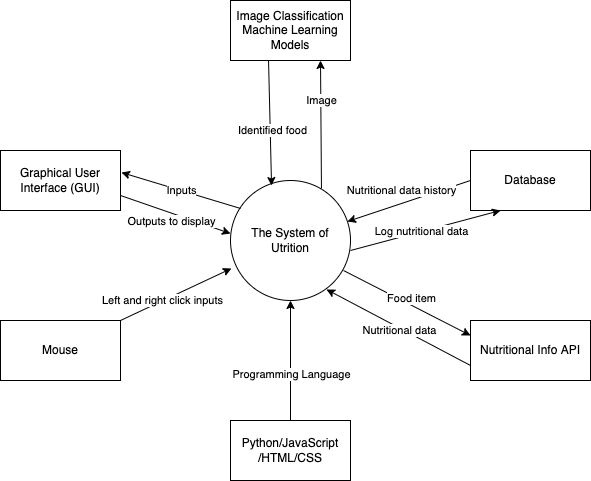
\includegraphics[scale=0.6]{work_context_diagram.png}
	\caption{Work Context Diagram}
\end{figure}


\subsubsection{Work Partitioning}

\begin{tabular}{ |p{5cm}|p{4cm}|p{6.5cm}| }
\hline
\textbf{Event Name}                   & \textbf{Input/Output}                                            & \textbf{Summary}                                                                                                                            \\ 
\hline
System receives image                 & User uploaded image (in) / Pre-processed image (out)             & User uploads an image and it is pre-processed into a format that can be sent to the computer vision algorithm.                              \\ 
\hline
Food identified in image              & Pre-processed image~(in) / Identified food (out)                 & The pre-processed image is processed to identify the food it represents through the use of our machine learning computer vision algorithm.  \\ 
\hline
Nutritional data retrieved            & Identified food(in) / Nutritional data (out)                     & The identified food is passed into a matching algorithm to retrieve the associated nutritional data from all stored nutritional data.       \\ 
\hline
Nutritional data displayed            & Nutritional data (in) / Visual display of nutritional data (out) & The raw nutritional data is transformed into a human readable format and displayed to the user.                                             \\ 
\hline
Nutritional data~logged               & Nutritional data (in) / Logging of data (out)                    & The nutritional data and search information of a user's search is internally logged and persists after the program has exited.              \\ 
\hline
Past nutritional data retrieved       & User mouse input (in) / Nutritional data (out)                   & The user is able to retrieve the nutritional data and search information of their past image uploads.                                       \\ 
\hline
Past nutritional data chart displayed & Nutritional data (in) / Chart (out)                              & Past nutritional data is displayed in a graph, showing past searches and nutritional data through various periods of time.                  \\
\hline
\end{tabular}

\subsubsection{Individual Product Use Cases}
\begin{figure}[H]
	\centering
	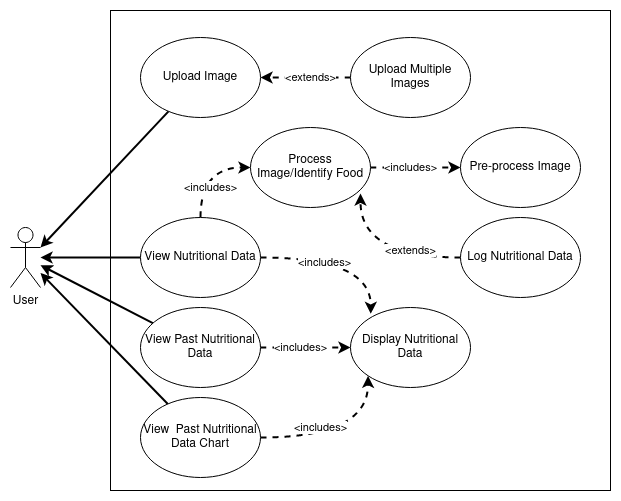
\includegraphics[scale=0.7]{use_case_diagram.png}
	\caption{Use Case Diagram}
\end{figure}

\subsection{Functional Requirements}

\FillFRNumber
\begin{itemize}
    \item \textit{Description}: The user shall have the ability to upload digital images of \textbf{standard image types} to the system. 
    \item \textit{Rationale}: In order for the system to identify the food a user is eating, the user would have to upload an image of their food to the system. The image shall be saved on the user’s device, which can then be selected.
    \item \textit{Priority}: High
\end{itemize}


\FillFRNumber
\begin{itemize}
    \item \textit{Description}: The user shall have the ability to upload multiple digital images of \textbf{standard image types} to the system.
    \item \textit{Rationale}: In order for the system to return the total nutritional content of a users meal, the user would have to upload multiple images of the individual components of their meal for the system to identify. The images shall be saved on the user’s device, which can then be selected.
    \item \textit{Priority}: Medium
\end{itemize}

\FillFRNumber
\begin{itemize}
    \item \textit{Description}: The system will be able to identify the type of food that is captured in an image. 
    \item \textit{Rationale}: In order for the system to return the nutritional content of a food, the system must first identify the food present in an image.
    \item \textit{Priority}: High
\end{itemize}

\FillFRNumber
\begin{itemize}
    \item \textit{Description}: The system will be able to store the nutrition facts of a variety of foods, including their macro-nutrients, micro-nutrients, and caloric details.
    \item \textit{Rationale}: In order to provide a user with the nutritional regarding their meal, the system must first be able to store the nutritional data for a large variety of foods for later use.
    \item \textit{Priority}: High
\end{itemize}

\FillFRNumber
\begin{itemize}
    \item \textit{Description}: The system will be able to retrieve the nutrition facts for a specific food.
    \item \textit{Rationale}: In order to provide the user with the nutritional data regarding their meal, the system would have to be able to retrieve the nutritional data for a given food.
    \item \textit{Priority}: High
\end{itemize}

\FillFRNumber
\begin{itemize}
	\item \textit{Description}: The system will log the nutritional data of a food.
	\item \textit{Rationale}: Nutritional data of a food will be saved for future reference. This system shall be able to fetch previously recorded data for other processes, such as displaying visuals and calculating nutritional summaries. 
	\item \textit{Priority}: Medium
\end{itemize}

\FillFRNumber
\begin{itemize}
	\item \textit{Description}: The user will be able to access the nutritional data of previously logged foods. 
	\item \textit{Rationale}: Nutritional data found in the database shall be available to be referenced and displayed to the user. This will allow the user to view nutritional details of the food that was previously tracked within the application. 
	\item \textit{Priority}: Medium
\end{itemize}

\FillFRNumber
\begin{itemize}
	\item \textit{Description}: The system will display the nutritional information of a food to the user. 
	\item \textit{Rationale}: Nutritional data of a particular food item shall be displayed on the user interface, so the user can view the nutritional breakdown of the food.
	\item \textit{Priority}: High
\end{itemize}

\FillFRNumber
\begin{itemize}
	\item \textit{Description}: The system will display the history of logged nutritional data in a graph. 
	\item \textit{Rationale}: Previously tracked nutritional statistics will be rendered in a graph as a function over time. This display will be a visual indicator of trends and overall progress.
	\item \textit{Priority}: Medium
\end{itemize}


\section{Nonfunctional Requirements}

\plt{List your nonfunctional requirements.  You may consider using a fit
  criterion to make them verifiable.}
\plt{The goal is for the nonfunctional requirements to be unambiguous, abstract
  and verifiable.  This isn't easy to show succinctly, so a good strategy may be
to give a ``high level'' view of the requirement, but allow for the details to
be covered in the Verification and Validation document.}
\plt{An absolute requirement on a quality of the system is rarely needed.  For
  instance, an accuracy of 0.0101 \% is likely fine, even if the requirement is
  for 0.01 \% accuracy.  Therefore, the emphasis will often be more on
  describing now well the quality is achieved, through experimentation, and
  possibly theory, rather than meeting some bar that was defined a priori.}
\plt{You do not need an entry for correctness in your NFRs.  The purpose of the
  SRS is to record the requirements that need to be satisfied for correctness.
  Any statement of correctness would just be redundant. Rather than discuss
  correctness, you can characterize how far away from the correct (true)
  solution you are allowed to be.  This is discussed under accuracy.}

\noindent \begin{itemize}

\item[NFR\refstepcounter{nfrnum}\thenfrnum \label{NFR_Accuracy}:]
  \textbf{Accuracy} \plt{Characterize the accuracy by giving the context/use for
    the software.  Maybe something like, ``The accuracy of the computed
    solutions should meet the level needed for $<$engineering or scientific
    application$>$.  The level of accuracy achieved by \progname{} shall be
    described following the procedure given in Section~X of the Verification and
    Validation Plan.''  A link to the VnV plan would be a nice extra.}

\item[NFR\refstepcounter{nfrnum}\thenfrnum \label{NFR_Usability}:] \textbf{Usability}
  \plt{Characterize the usability by giving the context/use for the software.
    You should likely reference the user characteristics section.  The level of
    usability achieved by the software shall be described following the
    procedure given in Section~X of the Verification and Validation Plan.  A
    link to the VnV plan would be a nice extra.}

\item[NFR\refstepcounter{nfrnum}\thenfrnum \label{NFR_Maintainability}:]
  \textbf{Maintainability} \plt{The effort required to make any of the likely
    changes listed for \progname{} should be less than FRACTION of the original
    development time.  FRACTION is then a symbolic constant that can be defined
    at the end of the report.}

\item[NFR\refstepcounter{nfrnum}\thenfrnum \label{NFR_Portability}:]
  \textbf{Portability} \plt{This NFR is easier to write than the others.  The
    systems that \progname{} should run on should be listed here.  When possible
    the specific versions of the potential operating environments should be
    given.  To make the NFR verifiable a statement could be made that the tests
    from a given section of the VnV plan can be successfully run on all of the
    possible operating environments.}

\item Other NFRs that might be discussed include verifiability,
  understandability and reusability.

\end{itemize}

\section{Non-Functional Requirements}

\subsection{Look and Feel Requirements}

\subsubsection{Appearance Requirements}

\begin{enumerate}[{LF}1. ]
	\item Utrition’s user interface will be clutterless.\\
	\textbf{Rationale:} Users must be able to access and read all parts of the user interface. \\
	\textbf{Fit Criteria:} The distance between user interface components must exceed 20 pixels.
\end{enumerate}

\subsubsection{Style Requirements}

\begin{enumerate}[{LF}2. ]
	\item Utrition’s style will be consistent throughout the different stages of accessing the user interface.\\
	\textbf{Rationale:} The appearance of Utrition will be more professional and consistent. \\
	\textbf{Fit Criteria:} Users will only be able to see $\pi$ when using Utrition. $\pi$ is the consistent font type
\end{enumerate}

\subsection{Usability and Humanity Requirements}

\subsubsection{Ease of Use Requirements}

\begin{enumerate}[{UH}1. ]
	\item The user interface will be easy to navigate. \\
	\textbf{Rationale:} Allows the user to efficiently learn and use Utrition.\\
	\textbf{Fit Criteria:} The user will be able to navigate to the main menu from any page in 2 clicks.
\end{enumerate}

\subsubsection{Personalization and Internationalization Requirements}

\begin{enumerate}[{UH}2. ] 
	\item Utrition will retain the user’s previously tracked information.\\
	\textbf{Rationale:} Users will be able to view their dietary habits and can make nutritional adjustments based on their observations.\\
	\textbf{Fit Criteria:} The user will be able to view their diet for the past $\pi$ days.
	
\end{enumerate}

\subsubsection{Learning Requirements}

\begin{enumerate}[{UH}3. ] 
	\item Utrition will be able to be used by people aged 14 and higher who have received no training on the product.\\
	\textbf{Rationale:} Utrition should be able to be used by all individuals who are concerned with their dietary habits.\\
	\textbf{Fit Criteria:} 90\% of a test panel of the target demographic should be able to upload their food and retrieve the nutritional facts for it in 2 minutes.
\end{enumerate}

\subsubsection{Understandability and Politeness Requirements}

\begin{enumerate}[start=4,label={UH\arabic*.}]
	\item Key information will be easy to understand on Utrition.\\
	\textbf{Rationale:} Users will be more likely to use the webapp if they are able to understand it efficiently.\\
	\textbf{Fit Criteria:} Every clickable object will have a diagram associated with it. Calories, fat, sodium, carbohydrates, sugar, and protein will have a diagram associated next to it.
	\item Utrition will not overwhelm the user with information.\\
	\textbf{Rationale:} The user is only concerned with the nutritional information and not the calculations leading up to it.\\
	\textbf{Fit Criteria:} All backend calculations, such as identifying the uploaded food and retrieving the nutritional information, will not be displayed to the user.
\end{enumerate}

\subsubsection{Accessibility Requirements}

\begin{enumerate}[{UH}6. ] 
	\item Utrition will be able to be used by deaf people.\\
	\textbf{Rationale:} Durum Wheat Semolina aims to allow as many individuals as possible to use Utrition.\\
	\textbf{Fit Criteria:} There will be no sound used by the Utrition web app. 
\end{enumerate}

\subsection{Performance Requirements}

\subsubsection{Speed and Latency Requirements}

\begin{enumerate}[start=1,label={PR\arabic*.}]
	\item Switching between different UI screens will be quick.\\
	\textbf{Rationale:} The user should not have to wait to access different parts of the Utrition web app.\\
	\textbf{Fit Criteria:} The time between the user’s click and the new UI displaying will not exceed 2 seconds.
	\item Identifying and displaying each food item will be done quickly.\\
	\textbf{Rationale:} The main use of the web app should not force the user to wait.\\
	\textbf{Fit Criteria:} After uploading a picture, Utrition will always display the calculated food item within 10 seconds in a test with multiple images.
	\item Displaying the calculated food’s nutritional value will be done quickly. \\
	\textbf{Rationale:} The secondary use of the web app should not force the user to wait. \\
	\textbf{Fit Criteria:} After viewing the calculated food item, Utrition will always display the nutritional facts within 5 seconds in a test with multiple images.
\end{enumerate}

\subsubsection{Safety-Critical Requirements}
\hspace{1.5cm}N/A

\subsubsection{Precision or Accuracy Requirements}

\begin{enumerate}[start=4,label={PR\arabic*.}]
	\item Identifying and displaying each food item will be done correctly. \\
	\textbf{Rationale:} The main use of the web app should provide the user with accurate information. \\
	\textbf{Fit Criteria:} In a test with multiple images, Utrition will identify and display the correct food with an average accuracy of 70\%.
	\item  The displayed nutritional facts will be correct. \\
	\textbf{Rationale:} The information given to the user should be accurate. \\
	\textbf{Fit Criteria:} In a test with multiple images, Utrition will display the correct nutritional information for the calculated food 100\% of the time.
\end{enumerate}

\subsubsection{Reliability and Availibility Requirements}

\begin{enumerate}[{PR}6. ] 
	\item Utrition will be available to all users at all times.\\
	\textbf{Rationale:} The user should be able to track their diet whenever they decide to eat. \\
	\textbf{Fit Criteria:} Since Utrition is a local webapp, the user will always be allowed to use Utrition unless their device is down.
\end{enumerate}

\subsubsection{Robustness or Fault-Tolerance Requirements}
\hspace{1.5cm}N/A

\subsubsection{Capacity Requirements}

\begin{enumerate}[{PR}7. ] 
	\item Utrition will allow $\pi$ images to be uploaded as a group.\\
	\textbf{Rationale:} The user will have to wait too long for the calculated results if more than $\pi$ images are uploaded at once. \\
	\textbf{Fit Criteria:} The user will not be able to upload more than $\pi$ photos.
\end{enumerate}

\subsubsection{Scalability or Extensibility Requirements}

\begin{enumerate}[{PR}8. ] 
	\item Utrition will have no limit to the size of the user base for its lifespan. \\
	\textbf{Rationale:} Utrition should be available to all individuals who are health conscious.\\
	\textbf{Fit Criteria:} Utrition is a local web app and does not depend on a server.
\end{enumerate}

\subsubsection{Longevity Requirements}

\begin{enumerate}[{PR}9. ] 
	\item Utrition is expected to operate indefinitely.\\
	\textbf{Rationale:} Nutritional food values will never change and people will always want ways to regulate their diet. \\
	\textbf{Fit Criteria:} Utrition will be available to use on github.
\end{enumerate}

\subsection{Operational and Environmental Requirements}

\subsubsection{Expected Physical Environment}
\begin{enumerate}[{OE}1. ] 
	\item Utrition will be used on any smart device with access to the “.jpg” photo format.\\
	\textbf{Rationale:} The user must be able to download Utrition and upload a photo to it. \\
	\textbf{Fit Criteria:} 100\% of the tested smart devices should be able to use all functionalities of the Utrition web app.
\end{enumerate}

\subsubsection{Requirements for Interfacing with Adjacent systems}
\hspace{1.5cm}N/A (BRING UP WITH GROUP) 

\subsubsection{Productization Requirements}
\begin{enumerate}[start=2,label={OE\arabic*.}]
	\item Utrition will be distributed on github as a public repository.\\
	\textbf{Rationale:} Utrition is free to be used by anyone.\\
	\textbf{Fit Criteria:} Users will be able to find and pull the repository into their personal device.
	\item Utrition will be able to be installed by any individual aged 14 or older after reading the installation guide on the Utrition github page.\\
	\textbf{Rationale:} Utrition should be accessible to all users. \\
	\textbf{Fit Criteria:} 95\% of a test panel will be able to install Utrition after reading the installation guide.
\end{enumerate}

\subsubsection{Release Requirements}

\begin{enumerate}[{OE}4. ] 
	\item Utrition will not have any updates after initial public release.\\
	\textbf{Rationale:} Food components and their nutritional value do not change over time.\\	\textbf{Fit Criteria:} Utrition’s git will receive no updates after initial release.
\end{enumerate}

\subsection{Maintainability and Support Requirements}

\subsubsection{Maintenance Requirements}
\begin{enumerate}[{MS}1. ] 
	\item New data can be given to improve Utrition’s AI at any point.\\
	\textbf{Rationale:} Utrition’s AI must be ready to improve itself whenever needed to ensure it can detect food at 70\% accuracy.\\	
	\textbf{Fit Criteria:} Any backend developer is able to successfully upload new data to Utrition’s AI at any time. 
\end{enumerate}

\subsubsection{Supportability Requirements}
\begin{enumerate}[{MS}2. ] 
	\item Support on how to install and use Utrition will be found on Utrition’s github page. \\
	\textbf{Rationale:} Users who are not technologically advanced should be able to use Utrition.\\	
	\textbf{Fit Criteria:} All users will be able to view the support manuals on how to install and use Utrition.
\end{enumerate}

\subsubsection{Adaptability Requirements}
\hspace{1.5cm}N/A (BRING UP WITH GROUP) 

\subsection{Security Requirements}

\subsubsection{Access Requirements}
\begin{enumerate}[{SR}1. ] 
	\item The entirety of Utrition can be accessed by all individuals. \\
	\textbf{Rationale:} The user has the flexibility to improve Utrition and the right to know what they’re downloading onto their computer.  \\	
	\textbf{Fit Criteria:} Anyone will be able to pull the open-source project from github
\end{enumerate}

\subsubsection{Integrity Requirements}
\begin{enumerate}[{SR}2. ] 
	\item Utrition will not crash when an abnormal photo format is uploaded to the app. \\
	\textbf{Rationale:} Users should not be punished for uploading the wrong photo format/Utrition should not crash by improper user input.\\	
	\textbf{Fit Criteria:}  Utrition will only allow photo uploads from images that have the file extension “.jpg”
\end{enumerate}

\subsubsection{Privacy Requirements}
\begin{enumerate}[{SR}3. ] 
	\item Utrition will store the user’s data locally.\\
	\textbf{Rationale:} Only the user should have to view their stored dietary habits. \\	
	\textbf{Fit Criteria:} Utrition can be used offline and will never communicate with other servers.
\end{enumerate}

\subsubsection{Audit Requirements}
\hspace{1.5cm}N/A (BRING UP WITH GROUP) 

\subsubsection{Immunity Requirements}
\hspace{1.5cm}N/A (BRING UP WITH GROUP) 

\subsection{Cultural or Political Requirements}

\subsubsection{Cultural Requirements}

\begin{enumerate}[{CP}1. ] 
	\item Utrition will not display any culturally insensitive content. \\
	\textbf{Rationale:} Culturally insensitive topics are irrelevant for what Utrition provides.\\	
	\textbf{Fit Criteria:} 95\% of the test panel agree that Utrition does not provide any culturally insensitive content to the user.
\end{enumerate}

\subsubsection{Political Requirements}
\hspace{1.5cm}N/A (BRING UP WITH GROUP) 

\subsection{Legal Requirements}
\subsubsection{Compliance Requirements}
\begin{enumerate}[{LR}1. ]
	\item Utrition follows Canada’s Anti-Spam Legislation Requirements for Installing Computer Programs \citep{CanadianInstall}.\\
	\textbf{Rationale:} Durum Wheat Semolina complies with the law, so no unneeded delays occur.\\
	\textbf{Fit Criteria:} No malicious software will be present in Utrition’s github repository.
\end{enumerate}
\subsubsection{Standards Requirements}
\begin{enumerate}[start=2,label={LR\arabic*.}]
	\item Durum Wheat Semolina follows Canada's "Guide for Publishing Open Source 
	Code" \citep{CanadianCode}.\\
	\textbf{Rationale:} To assist Durum Wheat Semolina in setting up the development environment for Utrition.\\
	\textbf{Fit Criteria:} Durum Wheat Semolina commit no infractions when following Canada’s guide.
	\item Durum Wheat Semolina will adhere to the PEP8 Python coding conventions.\\
	\textbf{Rationale:} Ensures code is consistent for the whole development team to work efficiently \\
	\textbf{Fit Criteria:} Pylint will be used after every pull request.
	\item Utrition is created following the standards set by the Google HTML/CSS Style Guide \citep{HTMLCSSStyle} and Google Java Style Guide \citep{JavaStyle}. \\
	\textbf{Rationale:} Ensures code is consistent for the whole development team to work efficiently \\
	\textbf{Fit Criteria:} Before every pull request, code will be reviewed to ensure no violations of the standards occur.
\end{enumerate}

\section{Project Drivers }

\subsection{The Purpose of the Project}

The purpose of the Utrition application is to help individuals learn more about maintaining a healthy lifestyle and assisting them in making wise decisions. This application is built for the users to learn more about what their meals consist of by breaking down the calories and nutrition facts of the food they intend on eating or purchasing.  

\subsection{The Stakeholders }
 
3.2.1 The Client –  

The client requesting this application is the instructor of the Software Engineering 4G06 classes Dr. Smith and the teaching assistants. This application is expected to be unique as compared to products in the market that attempt to tackle a similar problem as per the client's request.  

3.2.2 The Customers -  

The customers of Utrition are assumed to be health conscious individuals that are attempting to improve their daily eating habits. 

3.2.3 Other Stakeholders – Other stakeholders of the Utrition application consist of Grocery Stores, restaurants and gyms. These stakeholders are affected as the users of this program may switch their previous dynamic with these stakeholders due to their increase in knowledge of how many calories they are consuming. These dynamic changes consist of attending the gym more often to burn off extra calories, a preference to cook from home so restaurants may expect a decrease in customers and lastly Grocery stores stock may be affected due to an increase in knowledge of nutritional facts. 

\subsection{Mandated Constraints} 

As we wish to make the artificial intelligence as accurate as possible the application will only be trained for individual food items or ingredients rather than whole meals. For example, the user is expected to provide a picture of lettuce rather than a sandwich. This constraint is to ensure that the user gets an accurate estimate of exactly the nutritional value of their meal as the AI may not detect all separate food items in one picture. 

\subsection{Relevant Facts and Assumptions } 


A1: There is an assumption that the client will only take a picture of individual ingredients. 

A2: The client is also expected to have knowledge of the metric system as Utrition will be outputting nutritional value data in Calories.

A3: The user has an understanding of how to effectivley utilize web based applications

\section{Project Issues}

\subsection{Open Issues}
Below are open issues concerning the development of Utrition:
\begin{itemize}
	\item Depending on the amount of identified food image data our team can obtain, the accuracy of our food detection machine learning model may be low
	\item Currently, Utrition is planned to saved past user input. It is unknown how this will be done. Employing an account and password system for each user is added functionality that may be difficult to implement 
	\item One requirement states that past nutritional values of food will be stored for easy access when the system needs it again. When saving large amounts of nutritional data, processing could become slow for the entire system.
\end{itemize}

\subsection{Off-the-Shelf Solutions}
\subsubsection{Ready-Made Products}
After investigating the market, there are two ready-made solutions that provide similar functionality to Utrition. Firstly, the application \href{https://www.caloriemama.ai/#Categories}{Calorie Mama} is able to identify calories when a picture is uploaded of the user's meal. Although this implements some of Utrition's functionality, it fails to identify nutritional information or save any past calorie calculations.

Another product the team found to be similar to Utrition is \href{https://play.google.com/store/apps/details?id=ai.bite.biteapp&hl=en_US&gl=US}{Bitesnap}. This application will be able to identify food items, provide their corresponding nutritional information and calories, and store this information to provide eating insights for the user. Frequent reviews state that the system is not able to identify many foods provided in an image by the user. This means that the application's food database is small. Utrition will focus on creating a machine learning model that is able to identify a vast number of food items by supplying a large dataset of labelled food images. 

\subsubsection{Reusable Components}
Through research into libraries and APIs, the team has identified two systems that can be used for development of Utrition. Firstly, our team plans to create a machine learning model to identify different food items from an uploaded image. To do this the \href{https://www.tensorflow.org/}{TensorFlow} library can be used. This free and open-source library will all use to create and employ our machine learning model.

Secondly, Utrition must be able to return nutritional information about a food when an image of that food is uploaded. In order to retrieve this nutritional information, calls to \href{https://www.nutritionix.com/business/api}{Nutritionix API} can be made. Nutritionix contains data on a vast range of foods and their nutritional value. Using the free version, our team can make calls to this API to retrieve needed nutritional information.

\subsubsection{Products That Can Be Copied}
The team will be using datasets of labelled food images in order to train our machine learning model. These datasets can be freely obtained online and used in our development.

\subsection{New Problems}
N.A.

\subsection{Tasks}
\subsubsection{Project Planning}
Team members will follow a strict schedule to ensure the completion of Utrition. The team will work in 1 week Sprint cycles where tasks are distributed during the first meeting of the week (Monday at 6:30pm) and all tasks must be finished before that meeting the week after. There is also a scheduled progress meeting half-way through the Sprint (Thursday at 1:30pm) to give an update to the team on each person's progress and discuss any blocking issues. The team will create tasks each week based on the due dates provided in SFWRENG 4G06. This ensures that all deadlines are met.

\subsection{Migration to the New Product}
N.A.

\subsection{Risks}
\subsubsection{Low Productivity}
Working on a team with multiple developers creates the possibility that some people will not be productive and complete their assigned tasks. Missed work will cause a higher risk for an incomplete or inadequate final implementation. This risk can be identified when a developer is frequently missing deadlines and delivering poorly done work. To address this risk, the offending team member will be addressed directly by the group and asked about their opinion on possible solutions. This can include working on different areas of the project, asking for help when needed, etc.\newline
\textbf{Probability:} \%15

\subsubsection{Inadequate Implementation}
Due to the volume of requirements, the difficulty of the implementation, and the timeline of the project, there is a risk that the development team will not be able to create a good quality product. This includes partial implementation of features or hardcoded work arounds. To identify this risk before it becomes an issue, the development team hosts weekly progress meetings to ensure all members are proceeding smoothly. In the event that this risk is unavoidable, the team will alter the final goals of Utrition to remove unnecessary functionality.\newline
\textbf{Probability:} \%10

\subsubsection{Limited Time Frame}
Since Utrition's final implementation and documentation are required in less than 7 months, there is a risk that the project does not get completed. Every team member has additional work responsibilities outside of this project which could affect the time they have to work on Utrition. One sign that this risk poses a threat to the project is missed deadlines. This sign can be identified easily during the team's weekly meetings. If this risk becomes a problem, the team will apply an all-hands-on-deck approach where all unfinished work will be split up equally.\newline
\textbf{Probability:} \%8

\subsection{Costs}
Utrition will be development using free programming technologies and open-source libraries. This sets the current budget of the project to \$0. The plan for Utrition's availability is for users to download all code files from GitHub in order to run the system. In future development, hosting Utrition as a website will cost between the range of \$3.95 - \$16.95 per month.

The time cost for the project is calculated based on the number of developers and the duration of the project. Utrition will be development by 6 individuals who all can provide 10 hours every week. The duration of the project is set to 8 months. Using these values, the total amount of time needed to complete the project is 1920 hours and 320 hours per developer.

\subsection{User Documentation and Training}
\subsubsection{User Documentation Requirements}
Utrition will be available to users from GitHub. Inside the repository, the README file will contain instructions for the download and setup of Utrition. Any required software needed by the user to run Utrition will be specified in this file along with solutions to common installation errors. This file will also discuss all functionality of the system and provide instructions for the user to use Utrition. This section will act as the user manual. 

\subsubsection{Training Requirements}
There is no training needed for users to use Utrition. Any questions regarding usage of the system will be available in the user manual.

\subsection{Waiting Room}
In this section, requirements for future releases of Utrition are stated from highest to lowest priority. For a more in-depth explanation of each requirement, please refer to section 3 (Stretch Goals) inside the Problem Statement and Goals document.

\begin{itemize}
	\item [\FillFRNumber] The system must be accessible online as a website.\newline
	\textbf{Rationale:} Hosting Utrition online will make it easier for users to access the system. They can search for Utrition in an online search instead of downloading the project from GitHub.
	
	\item [\FillFRNumber] The system must be able to identify the individual foods inside a picture of a meal.\newline
	\textbf{Rationale:} If the system can identify visually apparent ingredients inside of a meal, the user will not need to upload pictures of each individual food item which will increase efficiency.
	
	\item [\FillFRNumber] Users must be able to save preset meal options consisting of one or many foods.\newline
	\textbf{Rationale:} Users can save selected foods together as meals so they can easily log this meal as eaten without needing to manually upload images of individual ingredients.
	
	\item [\FillFRNumber] Utrition will provide insights into the eating habits of the user such as what vitamins they should try to consume more of based on their previous inputs.\newline
	\textbf{Rationale:} By providing health insights, the system will become more useful to users by helping them improve their eating habits rather than solely tracking them.
	
	\item [NF?.] Once hosted online, Utrition must compute output with similar performance to the downloaded system within a 25\% margin of error.\newline
	\textbf{Rationale:} Hosting Utrition online should provide similar performance speeds compared to the local version so users experience the same enjoyment levels when using the system.
	
\end{itemize}

\subsection{Ideas for Solutions}

Below are some ideas for implementation of Utrition:

\begin{itemize}
	\item Create frontend display using HTML/CSS and JavaScript to connect to backend
	\item Backend can be implemented with Python
	\item Use \href{https://www.tensorflow.org/}{TensorFlow} library to create a machine learning model and train it with datasets of labelled food
	\item Use \href{https://www.nutritionix.com/business/api}{Nutritionix API} calls to retrieve nutrition facts of food items
\end{itemize}

\section{Likely Changes}   

\noindent \begin{itemize}

\item[LC\refstepcounter{lcnum}\thelcnum\label{LC_meaningfulLabel}:] 
With respect to the A1, the system currently assumes the uploaded pictures will 
show individual ingredients. In the future, a more sophisticated computer 
vision model can be added to differentiate individual ingredients from a meal.

\item[LC\refstepcounter{lcnum}\thelcnum\label{LC_meaningfulLabel}:] 
The system currently supports a model where the user uploads images of food to 
be evaluated. In the future, the system may allow the user to record their 
meals in real time and identify nutritional facts instantaneously.

\item[LC\refstepcounter{lcnum}\thelcnum\label{LC_meaningfulLabel}:] 
The system is currently designed to run locally on the user's device. In the 
future, the system can be hosted online, and allow users to request nutritional 
data from system servers.

\end{itemize}

\section{Unlikely Changes}    

\noindent \begin{itemize}

\item[ULC\refstepcounter{ulcnum}\theulcnum\label{ULC_meaningfulLabel}:] 
The user's past nutritional history will always be stored locally on the user's 
device. This will remain limit the number of requests in the event the system 
is hosted online. Furthermore, this allows to access their nutritional history 
offline.

\end{itemize}

\section{Traceability Matrices and Graphs}

The purpose of the traceability matrices is to provide easy references on what
has to be additionally modified if a certain component is changed.  Every time a
component is changed, the items in the column of that component that are marked
with an ``X'' may have to be modified as well.  Table~\ref{Table:trace} shows the
dependencies of theoretical models, general definitions, data definitions, and
instance models with each other. Table~\ref{Table:R_trace} shows the
dependencies of instance models, requirements, and data constraints on each
other. Table~\ref{Table:A_trace} shows the dependencies of theoretical models,
general definitions, data definitions, instance models, and likely changes on
the assumptions.

\plt{You will have to modify these tables for your problem.}

\plt{The traceability matrix is not generally symmetric.  If GD1 uses A1, that
  means that GD1's derivation or presentation requires invocation of A1.  A1
  does not use GD1.  A1 is ``used by'' GD1.}

\plt{The traceability matrix is challenging to maintain manually.  Please do
  your best.  In the future tools (like Drasil) will make this much easier.}

\afterpage{
\begin{landscape}
\begin{table}[h!]
\centering
\begin{tabular}{|c|c|c|c|c|c|c|c|c|c|c|c|c|c|c|c|c|c|c|c|}
\hline
	& \aref{A_OnlyThermalEnergy}& \aref{A_hcoeff}& \aref{A_mixed}& \aref{A_tpcm}& \aref{A_const_density}& \aref{A_const_C}& \aref{A_Newt_coil}& \aref{A_tcoil}& \aref{A_tlcoil}& \aref{A_Newt_pcm}& \aref{A_charge}& \aref{A_InitTemp}& \aref{A_OpRangePCM}& \aref{A_OpRange}& \aref{A_htank}& \aref{A_int_heat}& \aref{A_vpcm}& \aref{A_PCM_state}& \aref{A_Pressure} \\
\hline
\tref{T_COE}        & X& & & & & & & & & & & & & & & & & & \\ \hline
\tref{T_SHE}        & & & & & & & & & & & & & & & & & & & \\ \hline
\tref{T_LHE}        & & & & & & & & & & & & & & & & & & & \\ \hline
\dref{NL}           & & X& & & & & & & & & & & & & & & & & \\ \hline
\dref{ROCT}         & & & X& X& X& X& & & & & & & & & & & & & \\ \hline
\ddref{FluxCoil}    & & & & & & & X& X& X& & & & & & & & & & \\ \hline
\ddref{FluxPCM}     & & & X& X& & & & & & X& & & & & & & & & \\ \hline
\ddref{D_HOF}       & & & & & & & & & & & & & & & & & & & \\ \hline
\ddref{D_MF}        & & & & & & & & & & & & & & & & & & & \\ \hline
\iref{ewat}         & & & & & & & & & & & X& X& & X& X& X& & & X \\ \hline
\iref{epcm}         & & & & & & & & & & & & X& X& & & X& X& X& \\ \hline
\iref{I_HWAT}       & & & & & & & & & & & & & & X& & & & & X \\ \hline
\iref{I_HPCM}       & & & & & & & & & & & & & X& & & & & X & \\ \hline
\lcref{LC_tpcm}     & & & & X& & & & & & & & & & & & & & & \\ \hline
\lcref{LC_tcoil}    & & & & & & & & X& & & & & & & & & & & \\ \hline
\lcref{LC_tlcoil}   & & & & & & & & & X& & & & & & & & & & \\ \hline
\lcref{LC_charge}   & & & & & & & & & & & X& & & & & & & & \\ \hline
\lcref{LC_InitTemp} & & & & & & & & & & & & X& & & & & & & \\ \hline
\lcref{LC_htank}    & & & & & & & & & & & & & & & X& & & & \\
\hline
\end{tabular}
\caption{Traceability Matrix Showing the Connections Between Assumptions and Other Items}
\label{Table:A_trace}
\end{table}
\end{landscape}
}

\begin{table}[h!]
\centering
\begin{tabular}{|c|c|c|c|c|c|c|c|c|c|}
\hline
   &FR1& FR2&FR3&FR4&FR5&FR6&FR7&FR8&FR9\\ \hline
LF1& & x& & & & & x& x& x \\ \hline
LF2& & x& & & & & x& x& x \\ \hline
UH1& & x& & & & & & x& x \\ \hline
UH2& & & x& & & & x& & x \\ \hline
UH3& x& x& & & & & x& &  \\ \hline
UH4& x& x& & & & & x& x& x\\ \hline
UH5& x& x& & & & & x& x& x\\ \hline
UH6& x& x& & & & & & x& x\\ \hline
PR1& & & & & & & x& x& x\\ \hline
PR2& & & & & & & x& x& x\\ \hline
PR3& & & & & x& & & x& \\ \hline
PR4& & & x& x& x& & x& x& \\ \hline
PR5& & & & & & & & & \\ \hline
PR6& x& x& x& x& x& & x& x& x\\ \hline
PR7& & x& & & & & & & \\ \hline
PR8& & & & & & & & & \\ \hline
PR9& & & & & & & & &\\ \hline
OE1& & & & & & & & &\\ \hline
OE2& & & & & & & & &\\ \hline
OE3& & & & & & & & &\\ \hline
OE4& & & & & & & & &\\ \hline
MS1& & & x& & x& & & x&\\ \hline
MS2& & & & & & & & & \\ \hline
SR1& & & & & & & & & \\ \hline
SR2& x& x& & & & & & & \\ \hline
SR3& & & & x& & x& & & \\ \hline
CP1& & & & & & & & & \\ \hline
LR1& & & & & & & & & \\ \hline
LR2& & & & & & & & & \\ \hline
LR3& & & & & & & & & \\ \hline
LR4& & & & & & & & & \\ \hline
\end{tabular}
\caption{Traceability Matrix Showing the Connections Between FUNCTIONAL AND NON FUNCTIONAL}
\label{Table:A_trace}
\end{table}

\begin{table}[h!]
\centering
\begin{tabular}{|c|c|c|c|c|c|c|c|c|c|c|c|c|c|c|c|c|c|c|c|c|c|c|c|}
\hline        
	& \tref{T_COE}& \tref{T_SHE}& \tref{T_LHE}& \dref{NL}& \dref{ROCT} & \ddref{FluxCoil}& \ddref{FluxPCM} & \ddref{D_HOF}& \ddref{D_MF}& \iref{ewat}& \iref{epcm}& \iref{I_HWAT}& \iref{I_HPCM} \\
\hline
\tref{T_COE}     & & & & & & & & & & & & & \\ \hline
\tref{T_SHE}     & & & X& & & & & & & & & & \\ \hline
\tref{T_LHE}     & & & & & & & & & & & & & \\ \hline
\dref{NL}        & & & & & & & & & & & & & \\ \hline
\dref{ROCT}      & X& & & & & & & & & & & & \\ \hline
\ddref{FluxCoil} & & & & X& & & & & & & & & \\ \hline
\ddref{FluxPCM}  & & & & X& & & & & & & & & \\ \hline
\ddref{D_HOF}    & & & & & & & & & & & & & \\ \hline
\ddref{D_MF}     & & & & & & & & X& & & & & \\ \hline
\iref{ewat}      & & & & & X& X& X& & & & X& & \\ \hline
\iref{epcm}      & & & & & X& & X& & X& X& & & X \\ \hline
\iref{I_HWAT}    & & X& & & & & & & & & & & \\ \hline
\iref{I_HPCM}    & & X& X& & & & X& X& X& & X& & \\
\hline
\end{tabular}
\caption{Traceability Matrix Showing the Connections Between Items of Different Sections}
\label{Table:trace}
\end{table}

\begin{table}[h!]
\centering
\begin{tabular}{|c|c|c|c|c|c|c|c|}
\hline
	& \iref{ewat}& \iref{epcm}& \iref{I_HWAT}& \iref{I_HPCM}& \ref{sec_DataConstraints}& \rref{R_RawInputs}& \rref{R_MassInputs} \\
\hline
\iref{ewat}            & & X& & & & X& X \\ \hline
\iref{epcm}            & X& & & X& & X& X \\ \hline
\iref{I_HWAT}          & & & & & & X& X \\ \hline
\iref{I_HPCM}          & & X& & & & X& X \\ \hline
\rref{R_RawInputs}     & & & & & & & \\ \hline
\rref{R_MassInputs}    & & & & & & X& \\ \hline
\rref{R_CheckInputs}   & & & & & X& & \\ \hline
\rref{R_OutputInputs}  & X& X& & & & X& X \\ \hline
\rref{R_TempWater}     & X& & & & & & \\ \hline 
\rref{R_TempPCM}       & & X& & & & & \\ \hline
\rref{R_EnergyWater}   & & & X& & & & \\ \hline
\rref{R_EnergyPCM}     & & & & X& & & \\ \hline
\rref{R_VerifyOutput}  & & & X& X& & & \\ \hline
\rref{R_timeMeltBegin} & & X& & & & & \\ \hline
\rref{R_timeMeltEnd}   & & X& & & & & \\ 
\hline
\end{tabular}
\caption{Traceability Matrix Showing the Connections Between Requirements and Instance Models}
\label{Table:R_trace}
\end{table}

The purpose of the traceability graphs is also to provide easy references on
what has to be additionally modified if a certain component is changed.  The
arrows in the graphs represent dependencies. The component at the tail of an
arrow is depended on by the component at the head of that arrow. Therefore, if a
component is changed, the components that it points to should also be
changed. Figure~\ref{Fig_ATrace} shows the dependencies of theoretical models,
general definitions, data definitions, instance models, likely changes, and
assumptions on each other. Figure~\ref{Fig_RTrace} shows the dependencies of
instance models, requirements, and data constraints on each other.

% \begin{figure}[h!]
% 	\begin{center}
% 		%\rotatebox{-90}
% 		{
% 			\includegraphics[width=\textwidth]{ATrace.png}
% 		}
% 		\caption{\label{Fig_ATrace} Traceability Matrix Showing the Connections Between Items of Different Sections}
% 	\end{center}
% \end{figure}


% \begin{figure}[h!]
% 	\begin{center}
% 		%\rotatebox{-90}
% 		{
% 			\includegraphics[width=0.7\textwidth]{RTrace.png}
% 		}
% 		\caption{\label{Fig_RTrace} Traceability Matrix Showing the Connections Between Requirements, Instance Models, and Data Constraints}
% 	\end{center}
% \end{figure}

\section{Development Plan}

\plt{This section is optional.  It is used to explain the plan for developing
  the software.  In particular, this section gives a list of the order in which
  the requirements will be implemented.  In the context of a course  this is
  where you can indicate which requirements will be implemented as part of the
  course, and which will be ``faked'' as future work.  This section can be
  organized as a prioritized list of requirements, or it could should the
  requirements that will be implemented for ``phase 1'', ``phase 2'', etc.}

\section{Values of Auxiliary Constants}

\plt{Show the values of the symbolic parameters introduced in the report.}

\plt{The definition of the requirements will likely call for SYMBOLIC\_CONSTANTS.
Their values are defined in this section for easy maintenance.}

\plt{The value of FRACTION, for the Maintainability NFR would be given here.}

\newpage

\bibliographystyle {plainnat}

\bibliography {../../refs/References}

\newpage

\noindent \plt{The following is not part of the template, just some things to consider
  when filing in the template.}

\noindent \plt{Grammar, flow and \LaTeX advice:
\begin{itemize}
\item For Mac users \texttt{*.DS\_Store} should be in \texttt{.gitignore}
\item \LaTeX{} and formatting rules
\begin{itemize}
\item Variables are italic, everything else not, includes subscripts (link to
  document)
\begin{itemize}
\item \href{https://physics.nist.gov/cuu/pdf/typefaces.pdf}{Conventions}
\item Watch out for implied multiplication
\end{itemize}
\item Use BibTeX
\item Use cross-referencing
\end{itemize}
\item Grammar and writing rules
\begin{itemize}
\item Acronyms expanded on first usage (not just in table of acronyms)
\item ``In order to'' should be ``to''
\end{itemize}
\end{itemize}}

\noindent \plt{Advice on using the template:
\begin{itemize}
\item Difference between physical and software constraints
\item Properties of a correct solution means \emph{additional} properties, not
  a restating of the requirements (may be ``not applicable'' for your problem).
  If you have a table of output constraints, then these are properties of a
  correct solution.
\item Assumptions have to be invoked somewhere
\item ``Referenced by'' implies that there is an explicit reference
\item Think of traceability matrix, list of assumption invocations and list of
  reference by fields as automatically generatable
\item If you say the format of the output (plot, table etc), then your
  requirement could be more abstract
\end{itemize}
}

\section{Appendix}
This section has been added to the Volere template.
\begin{itemize}
	\item \textbf{Standard image types}: These are image files of extensions which include .png, .jpg, .jpeg.
\end{itemize}

\subsection{Constants}

\section{Reflection Appendix}
\subsection{Skills}
\subsubsection{Competence in Specialized Engineering Knowledge}
This skill describes one's knowledge on specialized engineering subjects in order to contribute to implementation, documentation, and the final presentation. Some examples of this knowledge include understanding each documents' purposes, the different software architectures to be used in implementation, and proper version control practices. This is highly important for the success of Utrition since all aspects of the project are technically advanced and could not be accomplished by individuals uneducated in software engineering. Ways for people to improve this skill include consulting notes from past courses taken, reviewing previous projects, and researching needed unknown areas of expertise.

\subsubsection{Effective Project Management}
Effective Project Management is a skill for planning and effectively managing a project’s time, resources, and scope. Also, to master the skill, one must be able to follow business practices when appropriate. In relation to Utrition, these business practices are: using git branches and pull requests, showing up to the biweekly meetings, working together on Microsoft Teams, and using git issues to assign tasks. Durum Wheat Semolina decided on these business practices, as they are needed to be able to allocate resources in an effective manner to ensure that the project tasks are efficiently completed. The most important business practice and the tool that assists Durum Wheat Semolina manage the project’s resources is git. There are many approaches to learning git. One of these approaches is to follow tutorials and guides online for how to effectively use git branches, issues, and pull requests. Another approach is to ask other members in Durum Wheat Semolina to teach the git business practices, as most software engineers have a profound understanding of git.
\subsubsection{Develops models/prototypes; tests, evaluates, \& iterates as 
appropriate}
This skill describes the ability to not only make changes to a system through 
successive iterations, but also completing analysis and evaluations of the 
system at each iteration. These practices help detect faults during the 
development process, before they can manifest as bugs, and helps ensure changes 
to the system adhere to the requirements. For Utrition, this is significant as 
it will be built out iteratively. Repeated, small changes will be made and 
include a set of tests to ensure that our project is meeting requirements 
throughout the development process. This skills can be exercised by creating a 
process for automated unit testing, as well as encouraging all team members to 
smoke test new code changes. Furthermore, the team can complete root cause 
analysis when fixing bugs in order to better track potentially error-prone code.

\subsubsection{Evaluates engineering tools, identifies their limitations, and selects, adapts, or extends them appropriately}
This skill describes the ability to choose the most effective software tool for an application from a variety of options based off of intended use, tool limitations, software requirements, ease of use, and a variety of other factors. Choosing the most relevant tools for our project is the best way to ensure that our project is not inherently limited by its framework and that it is ultimately successful. Knowing tool limitations will also allow us to adapt our product to either work around them or guide our development to incorporate them in our design process. The skill can be improved through reading tool documentation, researching tool reviews, comparisons, and benchmarks, and performing our own tests and sample code executions to evaluate their performance. 

\subsubsection{Active contribution to the planning and execution of a team project}
This skill describes the ability to contribute to the team project as an active member of the group. In order for all teammates to be more aligned with project goals and a standard of high-quality work, the group as a whole should be involved in the planning and execution of the project and be aligned on common goals. This requires the members to be invested in the planning and execution of the various components of the project. Having team members actively contribute to the project will foster a supportive and productive team dynamic. This skill can be improved through engaging in team meetings, sharing opinions or suggestions with the team, and helping with GitHub project board organization.

\subsection{Teammate Specific Learning Approaches}
\subsubsection{Alexander Moica}
Alexander has had repeated previous experience working with a specific set of software tools but has rarely branched out to investigate and evaluate potential alternatives. In order to develop the skills necessary for the efficient evaluation of competing software tools, Alexander will search for tool reviews, comparisons, and benchmarks. This method was chosen since this content is available in a variety of easily digestible formats - including visual representations, video reviews, and interactive comparison tables.

\subsubsection{Yasmine Jolly}
\subsubsection{Jeffrey Wang}
Jeffrey is familiar with the tools and programming languages frequently 
used in the academic setting, but needs to improve his self-directed learning 
ability. During the development of Utrition, there will be opportunities to 
handle new technology outside the scope of an academic setting that will 
require self-learning to understand (Section 16.1.1). Jeffrey will research 
unknown areas of expertise to quickly develop a understanding of the unknown 
area to a level adequate for this project. Furthermore, he will read the 
documentation of new technologies to better understand its capabilities. These 
methods were chosen as they best tackle learning about subjects outside the 
scope of an academic setting.
\subsubsection{Jack Theriault}
Jack has had experience with git, but he has not expanded on his knowledge and only knows the basic git commands for cloning, pulling, and pushing. In order for Jack to work effectively with Durum Wheat Semolina, Jack will need to follow tutorials and guides online on how to use the advanced git techniques. Jack has chosen this approach to learning because git is not difficult to understand with an online guide, and he does not want to distract his group mates with easy-to-answer questions.

\subsubsection{Catherine Chen}
Catherine expressed that she wanted to be more proactive in the planning and execution of the project. She has previously struggled with being aware of  what other members are working on. In order to develop her initiative and leadership skills, Catherine will lead project planning meetings. This includes spearheading team meetings for planning project deadlines, being aware of the allocation of tasks within the group, actively using GitHub issues, and project board organization. This method was chosen as it allows her to take more of a leadership role within the team where she can plan the allocation of tasks to team members, and she will gain a more holistic view on the project.
\subsubsection{Justina Srebrnjak}
Justina identifies that she has difficulty with understanding certain engineering tools such as \LaTeX, make, and certain programming languages such as JavaScript (Section 16.1.3). In order to better understand these tools as well as their limitations and uses, Justina will read any documentation available. She has chosen this method since she possesses a visual learning style and documentation is easily accessible online.

\end{document}
